\documentclass[onecolumn, 12pt]{book}

\usepackage[latin1]{inputenc}   
\usepackage{amsmath}
\usepackage{algorithm}
\usepackage{algorithmic} 
%\usepackage[T1]{fontenc}

%\usepackage[francais]{babel}     
\usepackage{layout}    
\usepackage[top=2cm, bottom=2cm, left=2cm, right=2cm]{geometry} 
\usepackage{setspace}
\usepackage{soul}
\usepackage{color} 
\usepackage{verbatim}
\usepackage{moreverb}
\usepackage{listings}
\usepackage{url}
\usepackage{graphicx}
\usepackage{epstopdf}
\usepackage{caption}
\usepackage{setspace}
 
 
% \title{Mod\`ele de Donn\'ees}
% \author{Willy Ehounou}
 %\date{01/06/15}
\title{Plan de th\`ese}
%\author{Jules \bsc{Verne}}
\date{\oldstylenums{1875}} 

\newtheorem{definition}{D\'efinition}
\newtheorem{theorem}{Theorem}
\newtheorem{claim}[theorem]{Claim}
\newtheorem{proposition}[theorem]{Proposition}
\newtheorem{lemma}[theorem]{Lemma}
\newtheorem{corollary}[theorem]{Corollary}
\newtheorem{conjecture}[theorem]{Conjecture}
\newtheorem{observation}{Observation}
\newtheorem{example}{Exemple}
\newtheorem{remark}{Remark}

 
\begin{document}
\maketitle
\tableofcontents

\chapter{Simulation des algorithmes sur des r\'eseaux th\'eoriques}

\section{Objectifs}
Les travaux r\'ealis\'ees dans cette partie ont pour but de montrer que les algorithmes propos\'es (couverture et correction) fournissent un graphe non orient\'e de distance de Hamming minimale lorsque la matrice d'adjacence de ce graphe contient plus de corr\'elations {\em fausses positives} que de corr\'elations {\em fausses n\'egatives} et peu d'erreurs de corr\'elations. Le nombre d'erreurs  doit \^etre inf\'erieur \`a $6$ pour une probabilit\'e de corr\'elations {fausses positives} sup\'erieure \`a $0.8$ . 
Pour se faire, nous montrons que les sommets, n'appartenant \`a aucune couverture (sommets $\in sommets\_1$) doivent \^etre corrig\'es avec la m\'ethode de {\bf permutation al\'eatoire minimum} afin d'avoir de meilleurs r\'esultats.

\section{D\'efinitions}
\begin{definition}
Une {\em erreur de corr\'elation} est l'existence ou l'absence de corr\'elation entre deux ar\^etes (ou arcs) lorsque, respectivement, il n'existe pas de corr\'elations ou il en existe une.
\newline
L'absence de corr\'elation (corr\'elation {\em fausse n\'egative}) est d\'esign\'ee par $0$ dans la matrice d'adjacence tandis que l'existence de corr\'elation (corr\'elation {\em fausse positive}) a une valeur $1$ dans cette matrice. 
\end{definition}

\begin{definition}
Une corr\'elation entre ar\^etes (ou arcs) est l'existence d'un sommet commun aux ar\^etes (ou arcs). Ce sommet commun peut \^etre source, destination ou interm\'ediaire comme present\'e dans la figure \ref{typeSommetEnCommun}
\begin{centering} 
\begin{figure}[htb!] 
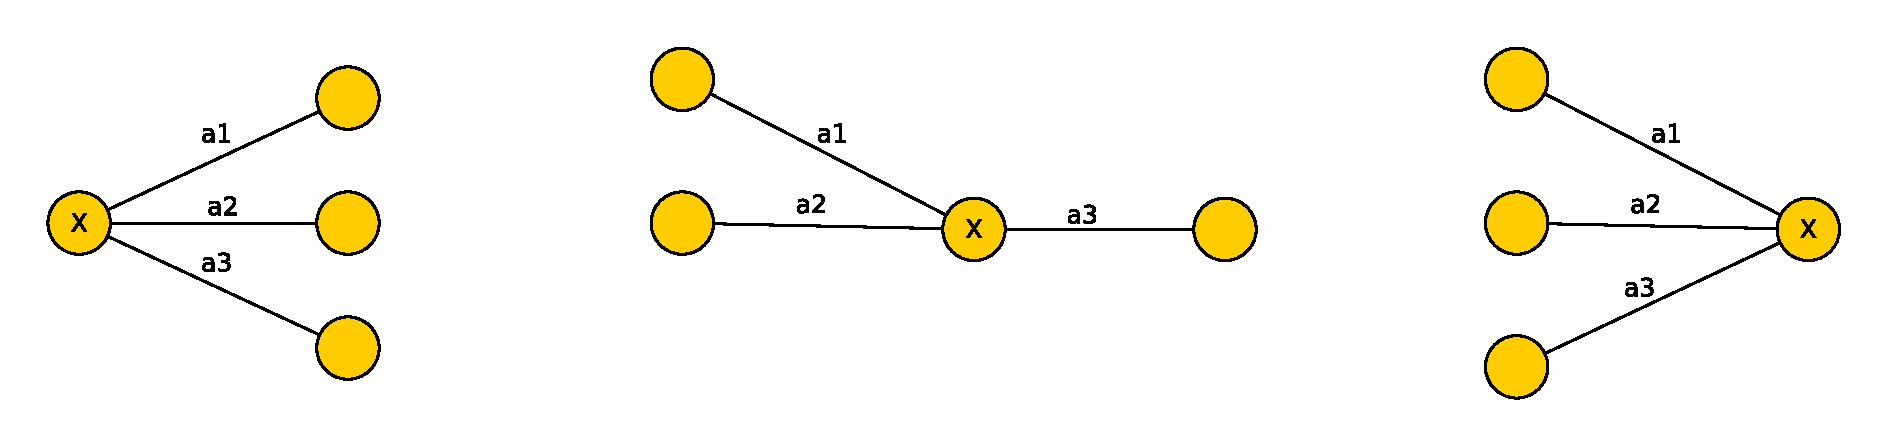
\includegraphics[scale=0.50]{images/typeSommetsEnCommun.eps}
\caption{De la gauche \`a la droite: sommet $X$ source, sommet $X$ interm\'ediaire, sommet $X$ destination}
\label{typeSommetEnCommun} 
\end{figure}
\end{centering} 
\end{definition}

\begin{definition}{ m\'etrique: distance de Hamming} \newline
La m\'etrique utilis\'ee pour diff\'erencier deux graphes est la {\em distance de Hamming}.
La distance de Hamming est le nombre d'ar\^etes (ou arcs) diff\'erentes entre deux graphes ayant le m\^eme ensemble de sommets. 
\end{definition}
Ainsi, une distance de Hamming \'egale \`a $0$ signifie que les deux graphes sont identiques. Tandis que  une distance de Hamming \'egale \`a $k$ signifie qu'il a $k$ ar\^etes diff\'erentes entre ces deux graphes.

\begin{definition}{ fonction de c\^out d'un sommet} \newline
La fonction de c\^out d'un sommet est le c\^out de chaque ar\^ete ajout\'ee ou supprim\'ee lorsqu'on applique l'algorithme de correction sur ce sommet.
\end{definition}
Le co\^ut d'une ar\^ete peut \^etre
\begin{itemize}
	\item unitaire : l'ajout et la suppression valent $1$.
	\item normal: la suppression est la probabilit\'e de l'ar\^ete et l'ajout vaut  $1$ moins cette probabilit\'e.
	\item carr\'e : la suppression est la probabilit\'e au carr\'e de l'ar\^ete et l'ajout vaut  $1$ moins cette probabilit\'e au carr\'e.
	\item quadratique :  la suppression est la probabilit\'e de l'ar\^ete \`a la puissance $4$ et l'ajout vaut  $1$ moins cette probabilit\'e \`a la puissance $4$.
\end{itemize}

\section{Donn\'ees: G\'en\'eration al\'eatoires de graphes} 
\subsection{G\'eneration de r\'eseaux de flots}
La structure de donn\'ees utilis\'ee, pour le graphe du r\'eseau de flots, est une {\em matrice d'adjacence}.
Cette matrice d'adjacence est une matrice carr\'ee de {\em n} sommets.
On d\'efinit le nombre de sommets {\em n} et le degr\'e moyen  $\alpha$ du graphe. 
La probabilit\'e d'existence d'une ar\^ete est de $proba = \frac{\alpha}{N}$.
Toutefois, si le graphe obtenu \`a partir de la matrice d'adjacence n'est pas connexe, on choisit al\'eatoirement un sommet de chaque composante connexe et on ajoute une ar\^ete entre ces sommets.
\newline
% orientation
Pour orienter les ar\^etes, on r\'ealise un tri topologique avec un parcours en largeur {\em Breath First Search (BFS)} du graphe non orient\'e g\'en\'er\'e, \`a partir de certains sommets choisis comme des sources. 
Chaque sommet $x$ a un ordre topologique $D_x$ et l'ar\^ete $a_{xy}$ devient soit l'arc $a_{xy}$ si $D_x < D_y$ soit l'arc $a_{yx}$ si $D_x > D_y$. 
Le graphe obtenu est alors orient\'e (un {\em Directed Acyclic Graph} $DAG$).
\newline
% ajout flots sur chaque arc
L'ajout des flots sur chaque arc se fait par un parcours en largeur (BFS).
On d\'efinit les valeurs minimales et maximales des grandeurs physiques. 
Ces valeurs sont s\'electionn\'ees selon le r\'eseau \'energ\'etique \`a mod\'eliser. 
\`A titre d'exemple, les valeurs choisies pour des grandeurs \'electriques sont: les intensit\'es $I = [150, 200 ]$, les tensions $U = [220, 250]$, les puissances $P = [ 33000, 62500]$. \newline
On d\'ebute par les sommets sources dont on g\'en\`ere une valeur al\'eatoire comprise dans l'un des intervalles de ces grandeurs. 
Chaque arc sortant du sommet source re\c coit  un flot \'egal \`a la somme des flots sur les arcs entrants du sommet source multipli\'ee par le facteur $\epsilon$ (d\'esignant les pertes joules) et divis\'ee par le degr\'e sortant de ce sommet si nous avons comme grandeurs les intensit\'es et les puissances.
Dans le cas de grandeurs comme les tensions, le flot de chaque arc sortant est le flot multipli\'ee par le facteur $\epsilon$. 
On propage les valeurs des grandeurs physiques jusqu'\`a ce qu'on arrive aux sommets puits.
L'application de ces r\`egles de flots permettent de v\'erifier la {\em loi de conversation des noeuds}.

\subsection{G\'en\'eration de line graphes sous jacent au r\'eseau de flots non orient\'e}
% nommage des aretes et kes ce que 2 aretes correles
Nous nommons les arcs du graphe et nous construisons la matrice de corr\'elation selon la notion de corr\'elation entre arcs ($0$ aucuns sommets en commun sinon $1$).
La matrice binaire de corr\'elation est la {\em matrice d'adjacence du line graphe} sous jacent au graphe non orient\'e de notre r\'eseau de flots g\'en\'er\'e. Cette matrice est sym\'etrique et est not\'ee $matE$. \newline
Si la matrice $matE$ ne contient {\em aucune erreur de corr\'elation} alors elle admet une couverture en cliques c'est-\`a-dire que chaque sommet est contenu dans deux cliques au maximum et chaque ar\^ete est couverte par une seule clique.
Dans le cas contraire, nous utilisons l'algorithme de correction afin de proposer une couverture pour chaque sommet n'appartenant \`a aucune clique. 
\newline
Notre but est de proposer une couverture en cliques des matrices $matE$ erron\'ees afin que 
la distance de Hamming entre le line graphe de matrice d'adjacence $matE$ et le line graphe g\'en\'ere soit minimum. 

\subsection{Prise en compte de l'erreur de corr\'elation dans la matrice $matE$}
On g\'en\`ere $500$ graphes de flots de $n = 30$ sommets ayant un degr\'e moyen $\bar d = 5$.
On en d\'eduit \'egalement $500$ line graphes de $150$ sommets.
On introduit trois param\`etres $k, p, prob$:
\begin{enumerate}
\item $k$ d\'esigne le nombre de corr\'elations erron\'ees \`a ajouter dans la matrice $matE$. Dans nos simulations, $k \in [1,9]$.
\item $p$ d\'esigne le type d'erreurs \`a r\'ealiser, soit corr\'elation {\em fausses positives} (ajout d'ar\^etes) soit corr\'elation {\em fausses n\'egatives} (suppression d'ar\^etes) soit les deux. Cette variable $p \in [0,1]$ varie par pas de $0.1$. Par exemple
	\begin{itemize}
	\item si $p=0$ $\rightarrow$ on supprime uniquement des ar\^etes dans le line graphe.
	\item si $p=0.5$ $\rightarrow$ on ajoute et supprime \'equiprobablement des ar\^etes.
	\item si $p=1.0$ $\rightarrow$ on ajoute uniquement des ar\^etes dans le line graphe.
	\end{itemize}
\item $prob$ d\'esigne la probabilit\'e associ\'ee \`a une corr\'elation selon le type d'erreurs effectu\'e dans $matE$. Ce param\`etre est important car les valeurs de corr\'elations calcul\'ees  ne sont pas binaires mais probabilistes. Nous en reparlerons dans la section \ref{fonctionDeCout}.
\end{enumerate}
%comment je modifie matE
Pour ajouter des erreurs \`a notre matrice $matE$ de corr\'elation correcte, on tire al\'eatoirement $k$ cases non encore modifi\'ees. Nous mettons chaque case et sa case sym\'etrique \`a $1$ si la probabilit\'e de la case (g\'en\'er\'e selon la loi uniforme) est inf\'erieure ou \'egale \`a $p$. Si cette case est d\'ej\`a \`a $1$, on choisit une autre case.
\newline
Nous d\'ecidons de modifier $k \in [1, 9]$ corr\'elations, selon $p=0.5$, dans la matrice $matE$ et nous appliquons les algorithmes de couverture et de correction.
\`A la fin de l'algorithme de couverture, s'il existe des sommets du line graphe non couverts par {\em une ou deux cliques}, on les ajoute \`a l'ensemble $sommets\_1$ et nous appliquons l'algorithme  de correction sur chaque sommet de $sommets\_1$ selon les m\'ethodes suivantes:
\begin{itemize}
\item m\'ethode 1 : degr\'e minimum avec remise.\newline
Elle consiste \`a s\'electionner le sommet de degr\'e minimum dans l'ensemble $sommets\_1$, \`a appliquer l'algorithme de correction afin de modifier $matE$ et enfin \`a re-ex\'ecuter les deux algorithmes sur la matrice $matE$ modifi\'ee.
\item m\'ethode 2 : co\^ut minimum avec remise. \newline
Elle consiste \`a s\'electionner le sommet de co\^ut minimum dans l'ensemble $sommets\_1$, \`a appliquer l'algorithme de correction afin de modifier $matE$ et enfin \`a re-ex\'ecuter les deux algorithmes sur la matrice $matE$ modifi\'ee.
\item m\'ethode 3 : co\^ut minimum avec permutation des sommets de $sommets\_1$. \newline
Elle consiste \`a choisir une permutation dont les sommets sont class\'es par ordre croissant de leur co\^ut  de modification de la matrice $matE$ et \`a appliquer l'algorithme de correction sur cette permutation.
\item m\'ethode 4 :  degr\'e minimum avec  permutation des sommets de $sommets\_1$. \newline
Elle consiste \`a choisir une permutation dont les sommets sont class\'es par ordre croissant de leur degr\'e et \`a appliquer l'algorithme de correction sur cette permutation.
\item m\'ethode 5 : permutation al\'eatoire des sommets de $sommets\_1$. \newline
Elle consiste \`a choisir al\'eatoirement $N$ permutations puis \`a appliquer l'algorithme de correction et \`a s\'electionner la permutation ayant un co\^ut et une distance de Hamming minimum.
\end{itemize}
% calcul de moy_dl et moy_dh
Consid\'erons 
%$k \in [1, 9]$ le nombre de corr\'elations d'ar\^etes modifi\'ees,
%  $\alpha \in [1, 5]$ le nombre de fois qu'on applique $k$ erreurs sur la matrice $matE_k$,  
% $LG_{k, \alpha}$ le line graphe dont on a modifi\'e $k$ corr\'elations d'ar\^etes $\alpha$ fois et 
% $LG'_{k, \alpha}$  le line graphe fourni par les algorithmes de couverture et de correction \`a partir du line graphe $LG_{k, \alpha}$.
 $k \in [1, 9]$ le nombre d'erreurs de corr\'elations dans $matE$,
  $\alpha \in [1, 5]$ le nombre de fois qu'on applique $k$ erreurs sur la matrice $matE_k$,  
 $LG_{k, \alpha}$ le line graphe dont on a modifi\'e $k$ corr\'elations $\alpha$ fois et 
 $LG'_{k, \alpha}$  le line graphe fourni par les algorithmes de couverture et de correction \`a partir du line graphe $LG_{k, \alpha}$.
 \newline
 On note les matrices d'adjacence de $LG_{k, \alpha}$ et $LG'_{k, \alpha}$ respectivement $matE_{k, \alpha}$ et $matE'_{k, \alpha}$.
\newline
En comparant
\begin{enumerate}
\item  $LG$ et $LG'_{k, \alpha}$, on obtient la distance de Hamming not\'ee $DH_{k,\alpha}$.
\item $LG_{k,\alpha}$ et $LG'_{k,\alpha}$, on a la distance line not\'ee $DL_{k,\alpha}$.
\end{enumerate}
On d\'efinit par les variables $moy\_DH$ et $moy\_DL$, les moyennes respectives des distances de Hamming (not\'ee $DH_{k,\alpha}$) et des distances line (not\'ee $DL_{k,\alpha}$) pour une valeur donn\'ee de $k$ et pour tout $\alpha \in [1, 5]$.
\begin{equation}
moy\_DH_k = \sum_{\alpha = 1}^{5} DH_{k, \alpha} \hspace{2 em}
moy\_DL_k = \sum_{\alpha = 1}^{5} DL_{k, \alpha}
\end{equation}

  
\section{R\'esultats}
% interpretation d'une distribution  DH et DL pour une methode
% presentation des differentes methodes et comparaison
% comparaison entre differentes p
% impact de la fonction de cout
Nous d\'ecrirons les distributions des distances line et de Hamming moyenn\'ees ($moy\_DL$ ou $moy\_DH$) pour une m\'ethode de correction (al\'eatoire) puis nous comparons les cinq m\'ethodes de correction en se basant sur les distances de Hamming moyenn\'ees. 
Nous expliquons le choix de la m\'ethode de {\em permutation al\'eatoire} et montrons que les algorithmes (couverture et correction) proposent de meilleurs r\'esultats lorsque la matrice de corr\'elation poss\`ede plus de corr\'elations {\em faux positives} que de corr\'elations {\em faux n\'egatives} et aussi peu d'erreurs de corr\'elations ($k < 6$). 
\newline
Nous pr\'esentons \'egalement l'impact de la fonction de co\^ut dans les distributions  de distances de Hamming.

\subsection{Distribution de la m\'ethode de permutation al\'eatoire}
% description distribution methode aleatoire
\begin{centering} 
\begin{figure}[htb!] 
\includegraphics[scale=0.10]{/home/willy/Documents/courbePython/courbeDegreCoutMinAleatoire_11_09_2017/permut_aleatoire_coutMin_degreMin_fct_cout_unitaire_500G/aleatoire/courbes/distanceMoyenDLDH_k_0_10_aleatoire_p_05.jpeg}
\caption{ M\'ethode permutation al\'eatoire avec co\^ut unitaire : distribution des distances line $moy\_DL$ et de Hamming $moy\_DH$ pour $k \in [1,  9]$ corr\'elations alter\'ees}
\label{distLineHammingPermutAleatoireK09p05} 
\end{figure}
\end{centering} 
\begin{centering} 
\begin{figure}[htb!] 
%\includegraphics[scale=0.09]{/home/willy/Documents/courbePython/courbeDegreCoutMinAleatoire_11_09_2017/permut_aleatoire_coutMin_degreMin_fct_cout_unitaire_500G/aleatoire/courbes/repartition_correlation_k_0_10_aleatoire_p_05_2D.jpeg}
\caption{ M\'ethode co\^ut minimum avec remise : fonction de repartition cumul\'ee des distances line $moy\_DL$ et de Hamming $moy\_DH$ pour $k \in [1, \cdots, 9]$ de corr\'elations alter\'ees}
\label{fctRepartitionCumuleDistLineHammingPermutAleatoireK09p05} 
\end{figure}
\end{centering} 
La figure \ref{distLineHammingPermutAleatoireK09p05} repr\'esente les histogrammes de la m\'ethode de permutation al\'eatoire pour une probabilit\'e $p=0.5$ et une fonction de c\^out normal $F_1$. \`A gauche de cette figure, nous avons les distributions des distances lines et \`a droite celle des distances de Hamming. Ces histogrammes partent d'une corr\'elation modifi\'ee (en haut de la figure \ref{distLineHammingPermutAleatoireK09p05}) \`a $9$ corr\'elations  modif\'ees (en bas de la figure \ref{distLineHammingPermutAleatoireK09p05}). 
\newline
Dans la repr\'esentation d'une distribution, chaque batonnet correspond au pourcentage de graphes associ\'e \`a une distance moyenn\'ee (line ou Hamming).
\`A titre d'exemple, pour $k=2$ corr\'elations modifi\'ees, le pic de l'histogramme est \`a $moy\_DL = 2$ pour les distances lines et de $moy\_DH=0$ pour les distances de Hamming. Les pourcentages de graphes pour  $moy\_DL = 2$ et $moy\_DH=0$ sont identiques c'est-\`a-dire $50\%$.
\newline
Nous avons, dans les histogrammes, une droite verticale $y = k$ (en rouge) correspondant \`a $k$ erreurs de corr\'elations.
On constate que les pics sont \`a gauche sur la droite $y = k$ pour $k \le 6$ corr\'elations modifi\'ees.
Cela signifie que le pourcentage de graphe dont $moy\_DL = k$  et $moy\_DH=0$ est le plus \'elev\'e (on retrouve en g\'en\'eral le line graphe initial) et entraine une asym\'etrie de la distribution des distances pour $k \le 6$.
En revanche, au d\'el\`a de $k>6$, l'algorithme de correction retrouve peu de corr\'elations modifi\'ees. Ce qui place le pic \`a droite de la droite $y = k$ et fournit une distribution gaussienne des distributions. \newline
Le fait que les distributions de distance line et de Hamming soient, toutes les deux, asym\'etriques (pour $k \le 6$) soient sym\'etriques (pour $k>6$) nous interrogent sur l'\'evolution des distributions de distance line par rapport \`a celle de Hamming. 
 Pour cela, on calcule leur corr\'elation par la fonction $F$ d\'efinie en \ref{formuleCorrelation} et dont la fonction de r\'epartition cumul\'ee est dans la figure \ref{fctRepartitionCumuleDistLineHammingPermutAleatoireK09p05}.
\begin{equation}
\label{formuleCorrelation}
F_{k, \alpha} = \frac{ | moy\_DL_{k, \alpha} - moy\_DH_{k, \alpha} | }{ max(moy\_DL_{k, \alpha},  moy\_DH_{k, \alpha}) }
\end{equation}
Si $moy\_DL$ et $moy\_DH$ \'evoluent de mani\`ere oppos\'e (l'un est sup\'erieur \`a $0$, l'autre est \'egal \`a $0$), la fonction $F$ est \'egale \`a $1$. Par contre, s'ils sont tr\`es corr\'el\'es (i.e \'evoluent identiquement) alors $F = 0$.
Ainsi lorsqu'elles \'evoluent dans le m\^eme ordre, on obtient la courbe racine carr\'ee. Tel est le cas dans la figure \ref{fctRepartitionCumuleDistLineHammingPermutAleatoireK09p05} pour $k > 6$. 
Les courbes tendent vers la fonction racine carr\'ee quand $k$ devient grand. 
Par ailleurs $F \approx 0$ quand $k$ est tr\`es petit (fig \ref{fctRepartitionCumuleDistLineHammingPermutAleatoireK09p05}, $k \le 6$).
\newline

\subsection{Comparaison des m\'ethodes de correction}
% comparer les differentes methodes selon la description sur la methode aleatoire
Nous recherchons la meilleure m\'ethode de correction parmi les cinq m\'ethodes \'enumer\'ees plus haut. 
Pour se faire, on dispose des distributions de distances line et de Hamming, des histogrammes, des fonctions de repartitions de ces distributions et aussi des moyennes de distances line/Hamming associ\'ees \`a $k$ corr\'elations \'erron\'ees pour chacune des m\'ethodes.  
Nous utilisons la moyenne des distances de Hamming pour la comparaison de m\'ethodes parce que la distance de Hamming permet d'\'evaluer la diff\'erence entre le graphe de base et celui pr\'edit par nos algorithmes.\newline
Rappelons qu'on a $p=0.5$ et la fonction de co\^ut est unitaire ($F_0$).
La figure \ref{compareDifferentesMethodesCorrectionSommets_fct_cout_unitaire_p05} affiche les courbes  des diff\'erentes m\'ethodes pour des distances de Hamming moyenn\'ees en fonction des $k$ erreurs de corr\'elations.
\newline
Nous constatons  que la pire des m\'ethodes est celle de degr\'e minimum avec remise (en rouge avec un rond) car elle est au dessus des autres et la meilleure est celle de {\em de permutation al\'eatoire} (en jaune avec un triangle) car elle propose des line graphes ayant  le nombre minimum d'ar\^etes diff\'erentes pour $ \forall k$.\newline
\begin{centering} 
\begin{figure}[htb!] 
% a changer par des chemins relatifs
\includegraphics[scale=0.25]{/home/willy/Documents/courbePython/courbeDegreCoutMinAleatoire_11_09_2017/comparaisonDifferentesMethodesFonctDeCout_normal_500G_p_05.jpeg}
\caption{ Comparaison des diff\'erentes m\'ethodes de correction de sommets pour $k \in [1,9]$ correlations modifi\'ees }
\label{compareDifferentesMethodesCorrectionSommets_fct_cout_unitaire_p05} 
\end{figure}
\end{centering} 
Nous retenons, pour la suite, la m\'ethode de permutation al\'eatoire comme m\'ethode de correction des sommets n'appartenant \`a aucune couverture (sommets $\in sommets\_1$).
\newline


\subsection{Influence des erreurs de corr\'elations sur les distributions}
% comparaison de p sur la methode de permutation aleatoire
\begin{centering} 
\begin{figure}[htb!] 
% meilleur probabilite p parmi les [0.0, 0.1, 0.2, ...., 1.0]
% a changer par des chemins relatifs
\includegraphics[scale=0.25]{/home/willy/Documents/courbePython/courbeDegreCoutMinAleatoire_11_09_2017/permut_aleatoire_coutMin_degreMin_fct_cout_normal_500G/aleatoire/courbes/comparaison_probabilities_p_00_10_moy_dh_aleatoire_p_10.jpeg}
\caption{ Comparaison des diff\'erentes probabilit\'es d'ajout $k \in [1,9]$ de corr\'elations fausses positives et fausses n\'egatives sur la m\'ethode de permutation al\'eatoire }
\label{compareDifferentesProbabilitesP0_1_fct_cout_unitaire_p05} 
\end{figure}
\end{centering} 

\begin{centering} 
\begin{figure}[htb!] 
% distribution de p = 1.0 
% a changer par des chemins relatifs
\includegraphics[scale=0.10]{/home/willy/Documents/courbePython/courbeDegreCoutMinAleatoire_11_09_2017/permut_aleatoire_coutMin_degreMin_fct_cout_normal_500G/aleatoire/courbes/distanceMoyenDLDH_k_0_10_aleatoire_p_10.jpeg}
\caption{ distribution des distances line et de Hamming pour $p=1.0$ et $k \in [1,9]$ correlations modifi\'ees}
\label{distributionDLDH_p1.0_k19_fct_cout_unitaire} 
\end{figure}
\end{centering} 

Faisons varier la variable $p \in [0,1]$ par pas de $0.1$ dans le but de visualiser l'impact de corr\'elations {\em fausses positives} et {\em fausses n\'egatives} dans l'ex\'ecution des algorithmes. Rappelons que l'ajout et la suppression d'ar\^etes ont le m\^eme co\^ut de traitement c'est-\`a-dire $1$.
La figure \ref{compareDifferentesProbabilitesP0_1_fct_cout_unitaire_p05} r\'esume l'\'evolution des types d'erreurs de corr\'elations ($p$) pour des distances de Hamming $moy\_DH$ en fonction de  $k \in [1, 9]$  erreurs de corr\'elations.
\newline 
Nous constatons que les algorithmes donnent de meilleurs r\'esultats pour $p = 1$ et de mauvais r\'esultats pour $p = 0$. 
En d'autres termes, lorsqu'on ajoute que des corr\'elations {\em fausses positives} i.e $p  = 1$ dans la matrice $matE$, les algorithmes  proposent, dans la majorit\'e des cas, un line graphe dont ces ar\^etes sont supprim\'ees. Cela s'illustre dans la figure \ref{distributionDLDH_p1.0_k19_fct_cout_unitaire} o\`u l'ajout de $5$ corr\'elations {\em fausses positives} influencent tr\`es peu les line graphes propos\'es puisqu'ils sont identiques aux line graphes initiales dans $45\%$ des cas. 
En revanche, ce pourcentage baisse avec beaucoup de corr\'elations {\em fausses positives}. Tel est le cas pour $k = 9$ corr\'elations o\`u le taux est de $24\%$. 
\newline
Par ailleurs, le mauvais r\'esultat obtenu pour des probabilit\'es $p < 0.5$ s'explique par la correction de tr\`es peu  de corr\'elations (inf\'erieure \`a $1/3$ des corr\'elations modifi\'ees) entrainant l'ajout d'ar\^etes au voisinage des sommets \`a traiter (sommets $\in sommets\_1$).
\newline
Nous pensons que le meilleur compromis est la probabilit\'e $p = 0.8$ parce que, pour peu de corr\'elations modifi\'ees ($k<5$), les lines graphes produits et g\'en\'er\'es diff\`erent de $k<5$ ar\^etes correspondant aux $k$ corr\'elations \'effectu\'ees  et au d\'ela $k \geq 5$, le nombre d'ar\^etes diff\'erentes est fonction du nombre de corr\'elations faites multipl\'e par $1.5$.
Cela signifie qu'il faut, dans la matrice de corr\'elation, $20\%$ de corr\'elations {\em fausses negatives} et $80\%$ de corr\'elation {\em fausses positives}. 
\newline
Que se passe-t-il si on priorise l'ajout de corr\'elations {\em fausses negatives} \`a chaque traitement c'est-\`a-dire la suppr\`ession d'ar\^etes.  Dans ce cas, l'ajout d'ar\^etes {\em fausses positives} a un co\^ut moins important que celui des {\em fausses negatives}. 
%Le co\^ut de traitement d'un sommet a-t-il un impact sur le graphe propos\'e?

\subsection{Impact de la fonction de co\^ut sur les distributions}
% urgent definir les fourchettes de probas pour chaque type de correlation
\label{fonctionDeCout}
\begin{centering} 
\begin{figure}[htb!] 
% a changer par des chemins relatifs
\includegraphics[scale=0.25]{/home/willy/Documents/courbePython/courbeDegreCoutMinAleatoire_11_09_2017/comparaisonDifferentesFonctDeCout_by_permut_aleatoire_p_05.jpeg}
\caption{ Comparaison des diff\'erentes fonction de co\^ut sur l'ajout de $k \in [1,9]$ de corr\'elations fausses positives et fausses n\'egatives pour une probabilit\'e $p = 0.5$ avec la m\'ethode de permutation al\'eatoire }
\label{compareDifferentesFonctionDeCout_p05} 
\end{figure}
\end{centering} 
Nous d\'efinissons quatre fonctions de co\^ut: unitaire (n=0), normal (n=1), carr\'e (n=2), quadratique (n = 4) selon l'expression suivante
\begin{equation}
	\begin{aligned}
	F_n = 
	\begin{cases}
		prob[(a_i,a_j)]^n   \\
		(1 - prob[(a_i,a_j)])^n \\
	\end{cases}
	\end{aligned}
\end{equation}
ou $prob[(a_i,a_j)]^n$, la corr\'elation entre les ar\^etes $a_i$ et $a_j$, correspond au co\^ut d'ajout de corr\'elations fausses n\'egatives, 
$(1-prob[(a_i,a_j)])^n$ au cout d'ajout de corr\'elations fausses positives.
\newline
\'Etant donn\'ee que nous avons utilis\'e des matrices binaires dans la g\'en\'eration de line graphes, nous assignons des probabilit\'es pour chaque type de corr\'elation tel que:
\begin{itemize}
\item $prob[(a_i,a_j)] = [0, 0.5[ $ : corr\'elation vrai n\'egative i.e $0 \rightarrow 0$
\item $prob[(a_i,a_j)] = [0.5, 0.79[ $: corr\'elation fausse n\'egative i.e $1 \rightarrow 0$
\item $prob[(a_i,a_j)] = 0.8 $ : corr\'elation fausse positive i.e $0 \rightarrow 1$
\item $prob[(a_i,a_j)] = ]0.8, 1] $ : corr\'elation vrai positive i.e $1 \rightarrow 1$
\end{itemize}
La figure \ref{compareDifferentesFonctionDeCout_p05} affiche les courbes des diff\'erentes fonctions de co\^ut en fonction de $k$ corr\'elations modifi\'ees pour $p = 0.5$.
\newline
Les $4$ courbes sont superpos\'ees pour $k\le5$ et au d\'el\`a de $k>5$, les courbes carr\'ee (n=2) et normal (n=1) ont les plus petites distances moyenn\'ees de Hamming.
Pour $k>9$, la courbe unitaire (n=0) \'evolue de mani\`ere exponentielle tandis que les courbes carr\'ee (n=2) et normal (n=1) ont un rapport de $2$ entre les distances de Hamming et le nombre $k$ de corr\'elations modifi\'ees.
On en d\'eduit que la pire fonction de co\^ut est la fonction unitaire (n=0 en jaune).
\newline
Toutefois, nous ne pouvons pas choisir la meilleure fonction de co\^ut car les fonctions des courbes {\em normal} et {\em carr\'e} \'evoluent identiquement.
 On peut conclure qu'utiliser les probabilit\'es de corr\'elations pour le calcul du co\^ut am\'eliore significativement les distances moyenn\'ees de Hamming.
 \newline
 On choisit pour la suite la fonction de cout normal $F_1$ pour le co\^ut de chaque ar\^ete. 





\end{document}